% \documentclass{article}
\documentclass[11pt,a4paper]{report}
\usepackage[english]{babel}
\usepackage[utf8]{inputenc}

% Graphics package
\usepackage{graphicx}
\graphicspath{ {images/} }

%Includes "References" in the table of contents
\usepackage[nottoc]{tocbibind}


% Latex commands
    \newcommand{\mat}[2][ccccccccccccccccccccccccccccccccccccccccccccc]{\left[
        \arraycolsep=1.2pt\def\arraystretch{1.5}
        \begin{array}{#1} #2 \\ 
        \end{array} 
        \right]}

        %% Miscelaneous commands
        
        %% Tool tracking positions
        \newcommand{\xbT}{\bf{x}{^b_T}} % tool tip in body coords
        \newcommand{\xwT}{\bf{x}{^w_T}} % tool tip in world coords
        \newcommand{\xcT}{\bf{x}{^c_T}} % tool tip in camera coords
        \newcommand{\xwE}{\bf{x}{^w_E}} % eraser in world coords
        \newcommand{\xcE}{\bf{x}{^c_E}} % eraser in camera coords

        \newcommand{\obT}{\bf{\theta}{^b_T}} % eraser in camera coords

        %% Tool tracking orientations
        \newcommand{\q}[3]{{^#1}\bf{q}{^#2_#3}} % eraser in world coords

        %% Rotation and Translation vectors
        \newcommand{\R}[2]{{^#1}{\bf{R}}{^#2}}
        \newcommand{\T}[2]{{^#1}{\bf{t}}{^#2}}


\begin{document}

\title{Final Progress Report}
\author{Lukas Gemar}
\date{March 4, 2016}
\maketitle

\begin{flushleft}

%%%%%%%%%%%%%%%%%%%%%%%%%%%%%%%%%%%%%%%%%%%%%%%%%%%%%%%%%%%%%%%%%%%%%%%%%%%%%%%
%%%%% Tool Model
%%%%%%%%%%%%%%%%%%%%%%%%%%%%%%%%%%%%%%%%%%%%%%%%%%%%%%%%%%%%%%%%%%%%%%%%%%%%%%%
\section{Tool Model}

\medskip

The position of the tip of the interaction tool is $ \xwT $. This position is specified in world coordinates; the superscript $w$ indicates that the coordinates of this position are specified relative to the origin of world space, $\bf{O_w}$. This origin of the world coordinate system is approximately the location of the users head. It is not exactly the location of the user's head because the user can look up and down and side to side while wearing the display. The origin of the world coordinate system should remain fixed to these rotations and translations. The rotation of the display is measured, but the translation of the display is not. However, the translation of the head should be a function of the rotation of the display. A simple model of how the head moves from side to side should relate the head's rotation to its movement relative to the neck and shoulders.

\medskip

Since the camera is mounted to the display, the position of the world coordinate system is not exactly the position of the camera. The origin of the camera coordinate system, $\bf{O_c}$, is offset from the world coordinate system by the rotation and translation of the user's head. Assuming that the rotation and translation of the user's head is in fact minimal while the user is seated, then the translation of the camera, $\T{c}{w}$, should be a function of the rotation of the head mounted display, $\R{c}{w}$: $\T{c}{w} = f(\R{c}{w})$. 

\medskip

Let $\R{c}{w}$ and $\T{c}{w}$ be the rotation and translation matrices, respectively, that specify the transformation from the world coordinate system to the camera coordinate system. Then the position of the interaction tool in camera coordinates, $ \xcT $,  is given by the following relation: 

\[ \xcT = \R{c}{w} \xwT + \T{c}{w} \]

The position of the tool relative to the camera, $ \xcT $, is not observed directly. However, this position is inferred from the position of the back of the tool, $ \xcE $, and the orientation of the tool. Call the back of the tool the eraser. The position of the eraser, $\xcE$, is found through computer vision. The orientation of the tool relative to the world coordinate systsem is specified by the orientation of the tool in body coordinates, $\obT$, and the rotation matrix from the body coordinates of the tool to the world coordinates, $\R{w}{b}$; their product yields the absolute orientation of the tool in world coordinates. To correctly display the orientation of the tool to the user, $\R{w}{b}$, the rotation of the camera relative to the world, must also be known. $\R{w}{b}$ is measured by the virtual reality display. The position of the tool in camera coordiantes is found through the following relation: 

\[ \xcT = \xcE + \R{c}{w}(\R{w}{b}\obT) \]

\medskip
%%%%%%%%%%%%%%%%%%%%%%%%%%%%%%%%%%%%%%%%%%%%%%%%%%%%%%%%%%%%%%%%%%%%%%%%%%%%%%%
%%%%% Camera Model
%%%%%%%%%%%%%%%%%%%%%%%%%%%%%%%%%%%%%%%%%%%%%%%%%%%%%%%%%%%%%%%%%%%%%%%%%%%%%%%
\section{Camera Model}

The following is a model of a single frame from the camera. In this frame, the red circular object represents the back of the interaction tool. The back of the interaction tool is called the eraser. The width of the target along the $x$ dimension of the image is $d_{u}$. 

\medskip

\begin{center}
    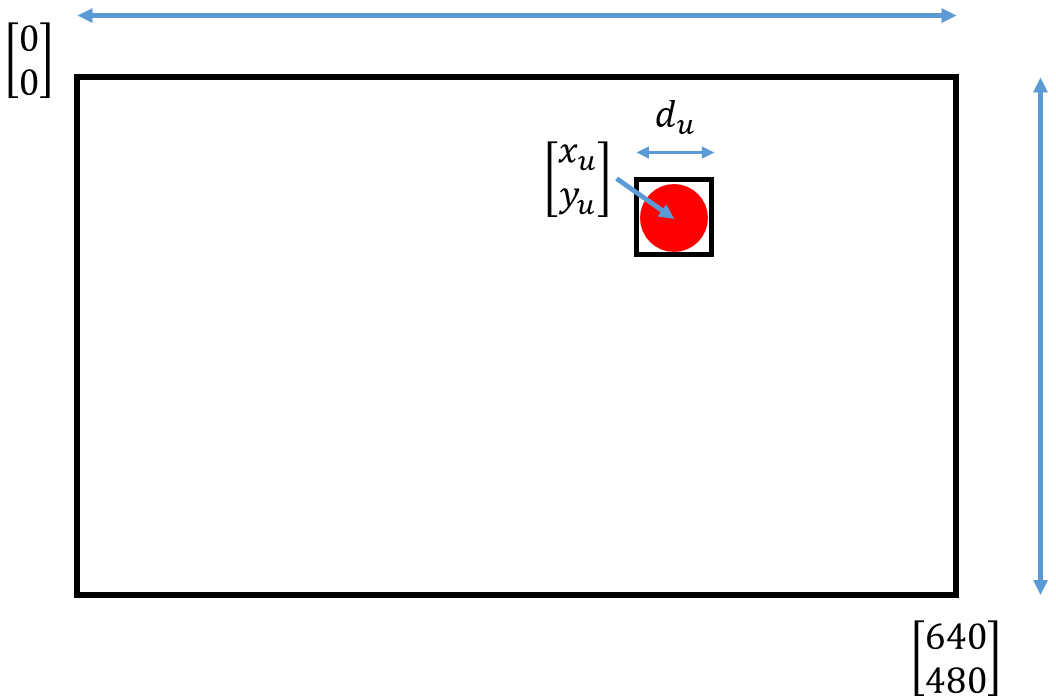
\includegraphics[scale=0.4]{computerVision}
\end{center}

\medskip

The midpoint of the eraser in the ideal undistorted image is $\bf{x^u_E} = \mat{ x_u & y_u }^{T}$. The center of the undistorted image is $c_x$ in the x direction and $c_y$ in the y direction. The focal lengths in the x and y directions are $f_x$ and $f_y$, respectively. These parameters are found through the camera calibration routine. The measurements of the center of the eraser and its width are related to the hidden state $\bf{\bf{x_C}} = \mat{ x_C & y_C & z_C }^{T}$ in the following way: 

\[
    \bf{\bf{y}} = h(\bf{\bf{x}})
        = \mat{x_u \\ y_u \\ d_{u} }
        = \mat{ \frac{f_x x_c}{z_c} + c_x \\ 
             \frac{f_y y_c}{z_c} + c_y \\ 
             \frac{d_c}{z_c \sqrt{\frac{1}{f_x^{2}} + \frac{1}{f_y^{2}}}}
           }
\]

These relationships are found through using a simple pin-hole camera model \cite{tsai_calibration}.

%%%%%%%%%%%%%%%%%%%%%%%%%%%%%%%%%%%%%%%%%%%%%%%%%%%%%%%%%%%%%%%%%%%%%%%%%%%%%%%
%%%%% Attitude Estimation
%%%%%%%%%%%%%%%%%%%%%%%%%%%%%%%%%%%%%%%%%%%%%%%%%%%%%%%%%%%%%%%%%%%%%%%%%%%%%%%
\section{Attitude Estimation}

The attitude of the interaction tool relative to the world coordinate frame can be represented in a number of ways. The two representations that will be important here are the attitude matrix and the attitude quaternion. First, the attitude of the orientation tool can be described by the attitude matrix $A$. The attitude matrix typically maps a vector in the reference frame to a vector in the the body frame \cite{Markley2007}. This mapping is given by the relation, 

\[ \bf{b} = A \bf{r} \]

Second, the attitude of the interaction tool can be represented as a quaternion. A rotation in three-dimensions is equivalent to an axis of rotation and and angle of rotation. If $\hat{n}$ is the axis of a rotation and $\theta$ is the angle of the rotation, then the quaternion $\overline{q}$ represents the attitude: 

\[ \overline{q} = \mat{\vec{q} \\ q_4} \] 

with $\vec{q} = \hat{n} \sin{\frac{\theta}{2}}$ and $q_4 = \cos{\frac{\theta}{2}}$. The quaternion must have length 1: $\overline{q}^T \overline{q} = 1$. 

The attitude matrix and the quaternion representing attitude are related by the following equation, where $A$ is a function of $\overline{q}$ \cite{Shuster1982}: 

\[ A(\overline{q}) = (q_4^2 - {\| \vec{q} \|}^2) I_{3x3} + 2 \vec{q}\vec{q}^2 - 2 q_4 \vec{q}{^X} \]

where $\vec{q}{^X}$ is the skew-symmetric cross product matrix, 

\[ \vec{q}{^X} = \mat{ 0 & -q_3 & q_2 \\ q_3 & 0 & -q_1 \\ -q_2 q_1 0} \]

The relationship between $A$ and $\overline{q}$ can also be expressed as the product of two matrices \cite{Markley2007}: 

\[ A(\overline{q}) = \Omega(\overline{q})^{T} \Phi(\overline{q}) \]

with 

\[ \Omega(\overline{q}) = \mat{q_4 \bf{I}_{3x3} + \overline{q}{^X} \\ -\overline{q}^T } \]

\[ \Phi(\overline{q}) = \mat{q_4 \bf{I}_{3x3} - \overline{q}{^X} \\ -\overline{q}^T } \]

%%%%%%%%%%%%%%%%%%%%%%%%%%%%%%%%%%%%%%%%%%%%%%%%%%%%%%%%%%%%%%%%%%%%%%%%%%%%%%%
%%%%% Bibliography
%%%%%%%%%%%%%%%%%%%%%%%%%%%%%%%%%%%%%%%%%%%%%%%%%%%%%%%%%%%%%%%%%%%%%%%%%%%%%%%
\bibliographystyle{unsrt}
\bibliography{references}

%%%%%%%%%%%%%%%%%%%%%%%%%%%%%%%%%%%%%%%%%%%%%%%%%%%%%%%%%%%%%%%%%%%%%%%%%%%%%%%
%%%%% End of the document
%%%%%%%%%%%%%%%%%%%%%%%%%%%%%%%%%%%%%%%%%%%%%%%%%%%%%%%%%%%%%%%%%%%%%%%%%%%%%%%

\end{flushleft}
\end{document}

